\documentclass[12pt]{article}

% Packages
\usepackage[T1]{fontenc}
\usepackage[margin=1in]{geometry}
\usepackage{amsmath,amssymb}
\usepackage[numbers,sort&compress]{natbib}
\usepackage{graphicx}
\usepackage{booktabs}
\usepackage{xcolor}
\usepackage{hyperref}
\graphicspath{{../../../figures/}}

\title{Supplementary Materials for:\\Observational evidence for a meter or more of sea-level rise by 2100}
\author{Minchew et al.}
\date{}

\begin{document}
\maketitle

%% ================================================================
%% MATERIALS AND METHODS
%% ================================================================
\section*{Materials and Methods}

\subsection*{GMSL rate estimates}

The satellite-era GMSL rates and 90\% confidence intervals reported in Figure~1 are derived from the quadratic trajectory methodology of Hamlington et~al.~\citep{Hamlington2024}. A quadratic is fit to the NASA satellite altimetry record (1993--2023) and the instantaneous rate at any time $t$ is given by $\dot{H}(t) = a + bt$, where $a$ and $b$ are the linear and quadratic coefficients. The 90\% confidence intervals are determined via a 10,000-member Monte Carlo simulation in which each realization perturbs the rate and acceleration by three independent error sources: (i)~serially correlated residuals after removing the quadratic trajectory, following Maul \& Martin~\citep{Maul1993}; (ii)~glacial isostatic adjustment (GIA) uncertainty from a Bayesian inversion of ice loading histories; and (iii)~satellite mission-specific measurement errors including altimeter noise, orbit determination, wet troposphere corrections, and inter-mission biases. The resulting 90\% CIs at the endpoints of the record are $2.1 \pm 1.0$~mm\,yr$^{-1}$ at 1993 and $4.5 \pm 1.0$~mm\,yr$^{-1}$ at 2024.

The pre-satellite rate of 1.1~mm\,yr$^{-1}$ (0.8--1.3~mm\,yr$^{-1}$, 90\% CI) averaged over 1900--1940 is computed from the Frederikse et~al.~\citep{Frederikse2020} tide-gauge reconstruction using a local polynomial regression (tricube kernel, 30-year bandwidth) that estimates instantaneous rates and their standard errors at each year. The narrower confidence interval reflects the longer averaging period and the lower sensitivity of tide-gauge uncertainties to the error sources that dominate the satellite record. Temperature changes between rate-doubling epochs are from Berkeley Earth \citep{Rohde2020}.

\subsection*{Observational datasets}

All component models are calibrated against published observational products (Table~S1). We use:
\begin{itemize}
\item \textbf{Global mean sea level:} NASA satellite altimetry (TOPEX/Jason, 1993--present; Hamlington et~al.~\cite{Hamlington2020}), with the Frederikse et~al.~\citep{Frederikse2020} tide-gauge reconstruction (1900--2018) and Dangendorf et~al.~\citep{Dangendorf2019} reconstruction for pre-satellite validation.
\item \textbf{Ocean thermal expansion:} NOAA thermosteric sea level, 0--700\,m (1955--2025) and 0--2000\,m (2005--2025) \citep{Levitus2012}. A 14\% structural uncertainty is applied to account for the documented low bias from vertical interpolation of sparse profiles \citep{Li2022}. Depth corrections for 700--2000\,m ($0.15 \pm 0.05$~mm\,yr$^{-1}$; \cite{Levitus2012, Cheng2017}) and below 2000\,m ($0.07 \pm 0.04$~mm\,yr$^{-1}$; \cite{Purkey2010, Desbruyeres2016}) are applied cumulatively for years before full-depth data are available.
\item \textbf{Glaciers:} GlaMBIE global consensus (2000--2024; GlaMBIE~\cite{GlaMBIE2024}), combining glaciological field measurements, satellite altimetry, DEM differencing, and GRACE/GRACE-FO gravimetry across all 19 RGI regions.
\item \textbf{Greenland:} Mouginot et~al.~\citep{Mouginot2019} SMB and discharge (1972--2018), with Mankoff et~al.~\citep{Mankoff2021} (1986--2023) withheld for validation. Subsurface ocean temperature from EN4 (200--500\,m, Greenland peripheral waters; Good et~al.~\cite{Good2013}). Surface temperature from Berkeley Earth \citep{Rohde2020}.
\item \textbf{Antarctica:} IMBIE satellite-era mass balance (1992--2020; Otosaka et~al.~\cite{Otosaka2023}), partitioned by region.
\item \textbf{Terrestrial water storage:} Frederikse et~al.~\citep{Frederikse2020} reconstruction (1900--2018).
\end{itemize}

\subsection*{Component models}

\paragraph{Thermosteric.} NOAA observations with literature depth corrections (hindcast, 1950--2020) are spliced with IPCC AR6 \texttt{oceandynamics} projections (2020--2150; Fox-Kemper et~al.~\cite{Fox-Kemper2021}). The IPCC projections are generated from a two-layer energy balance model \citep{Geoffroy2013} emulated by FaIR \citep{Smith2021}, with the ensemble filtered against observed global temperature and ocean heat content. Monte Carlo samples (2000) are drawn from the IPCC 107-quantile distributions using rank-preserving uniform draws, level-matched to observations at 2020.

\paragraph{Glaciers.} The rate of glacier sea level contribution is modeled as $\dot{H}_{\mathrm{gl}} = b\,T + c$, where $T$ is GMST anomaly, calibrated against GlaMBIE using Bayesian inference with weakly informative priors. A quadratic term $a\,T^2$ is included in the prior but the posterior is centered near zero, confirming linearity over the observed range. Cumulative loss is capped at total glacier volume.

\paragraph{Greenland SMB.} Observed RACMO-derived SMB \citep{Mouginot2019} for the hindcast. Forecasts use a quadratic temperature scaling $\Delta\dot{H}_{\mathrm{smb}} = C_T\,\Delta T + C_{T^2}\,\Delta T^2$ with sensitivities drawn from the inter-RCM spread \citep{Fettweis2020, Noel2021, Glaude2024}. The linear sensitivity $C_T \sim \mathcal{N}(-200, 80^2)$~Gt\,yr$^{-1}$\,$^\circ$C$^{-1}$ of GMST encompasses the MAR, RACMO, and HIRHAM estimates.

\paragraph{Greenland discharge.} Time-delay model (Eq.~1) calibrated against Mouginot et~al.~\citep{Mouginot2019} discharge by weighted least squares with BIC-weighted mixing across candidate delays $\delta \in \{4, 5, 6, 7, 8\}$~yr. Ocean temperature forcing under SSP scenarios is obtained from an independently calibrated linear transfer function mapping surface temperature to EN4 subsurface temperature. Each Monte Carlo sample draws a single set of physical parameters $(\gamma, r_0, \delta, \alpha, \beta)$ and evaluates all SSP scenarios under that draw, so that inter-SSP differences isolate the effect of the emissions pathway from parameter uncertainty.

\paragraph{WAIS.} Scenario-mixture framework with three outcomes weighted by assessed probabilities: (S1)~continued present-day rates extrapolated from IMBIE, (S2)~MISI-driven acceleration (15--100~cm) with trajectory exponent and right-skewed uncertainty from grounding-line flux nonlinearity \citep{Robel2019, Schoof2007}, (S3)~MISI plus additional cliff instability. The S2 lower bound is anchored to transient-calibrated ice sheet model projections: Goldberg et~al.~\citep{Goldberg2026} constrained two independent models against observed surface elevation changes at Thwaites and found $V_{af}$ loss rates of 180--200~Gt/a by 2067 from the trunk subdomain alone, using $n = 3$ with no calving or subglacial hydrology. Integrating this trajectory to 2100, scaling to the full Thwaites catchment, and adding comparable contributions from Pine Island Glacier (33~km grounding-line retreat since 1992; Rignot et~al.~\cite{Rignot2026}), Smith/Kohler, and S1-like non-ASE basins gives a conservative total of 13~cm; the 15~cm floor accounts for the known low biases in the underlying models. Within each scenario, the 2100 endpoint is drawn from a skew-normal distribution in log-space. The log-space formulation is motivated by the multiplicative structure of the dominant uncertainties (bed geometry, basal friction, ocean thermal forcing, buttressing loss all enter as multiplicative factors on grounding-line flux $q_g \propto h_g^{\,s}$), by the positivity constraint on mass loss, and by scale invariance across scenarios spanning two orders of magnitude. The skew-normal extension captures the asymmetry arising from flux nonlinearity \citep{Robel2019}. A multiplicative rheology correction $\sim\mathcal{N}(1.28, 0.07^2)$ is applied to all scenarios \citep{Martin2026, GetraerMorlighem2025}.

\paragraph{EAIS, Peninsula.} Bayesian rate--temperature models calibrated against IMBIE regional records \citep{Otosaka2023}. EAIS is dominated by accumulation increase under warming; the Peninsula by combined SMB and discharge. EAIS is excluded from the forecast sum because the 28-year satellite record cannot reliably distinguish the accumulation response from interannual variability ($R^2 = 0.57$), making forward projections poorly constrained. The EAIS contribution is small ($-13$ to $-30$~mm at 2100, depending on scenario) and its exclusion is conservative---it would reduce the total forecast if included.

\subsection*{Budget closure diagnostic}

The residual between the component sum and NASA altimetry is distributed across components in proportion to their variances: $\mathrm{shift}_i = (\sigma_i^2 / \sum_j \sigma_j^2) \times r$, where $r$ is the total residual and $\sigma_i$ is the standard deviation of component $i$ from its Monte Carlo ensemble. This is the Bayesian posterior update under joint Gaussian assumptions, applied as a diagnostic without modifying the component posteriors. The shift-to-sigma ratio for each component tests whether the implied adjustment is within the stated uncertainty.

\subsection*{Temperature scenarios}

SSP temperature trajectories (SSP1-2.6, SSP2-4.5, SSP3-7.0, SSP5-8.5) are from IPCC AR6 assessed warming projections. Historical forcing uses Berkeley Earth monthly GMST \citep{Rohde2020}. All anomalies are relative to a 1995--2005 baseline ($\approx$2005 reference year). Forecasts extend from 2020 to 2150, with pre-2020 values from the observational record.


%% ================================================================
\subsection*{Budget closure and validation}

Each component is calibrated independently; the total sea level is a diagnostic sum, not a calibration target. We evaluate budget closure by comparing the temperature-forced component hindcast (excluding EAIS; see main text) against NASA satellite altimetry over three epochs (Table~\ref{tab:budget_closure}).

\begin{table}[h]
\centering
\caption{Budget closure: component-sum rate versus NASA GMSL rate over three epochs. All rates from linear fits to the temperature-forced hindcast (no EAIS) and NASA altimetry.}
\label{tab:budget_closure}
\begin{tabular}{lcccr}
\toprule
Epoch & NASA (mm\,yr$^{-1}$) & Sum (mm\,yr$^{-1}$) & Residual (mm\,yr$^{-1}$) & Closure \\
\midrule
1993--2025 & 3.29 & 2.96 & 0.33 & 89.9\% \\
2000--2025 & 3.49 & 3.28 & 0.21 & 94.0\% \\
2010--2025 & 4.11 & 3.60 & 0.51 & 87.5\% \\
\bottomrule
\end{tabular}
\end{table}

A variance-weighted attribution distributes the residual across components in proportion to their uncertainties (Fig.~\ref{fig:budget_closure}). The thermosteric component absorbs the largest share (61\%), consistent with the known low bias in the NOAA product \citep{Li2022, Cheng2017}. Terrestrial water storage absorbs 21\%, reflecting poorly characterized structural uncertainty in groundwater and reservoir reconstructions. All components are within 1.3 standard deviations of their independent estimates. The framework closes the observed budget without requiring any component to depart from what the observations support.

\begin{figure}[h]
\centering
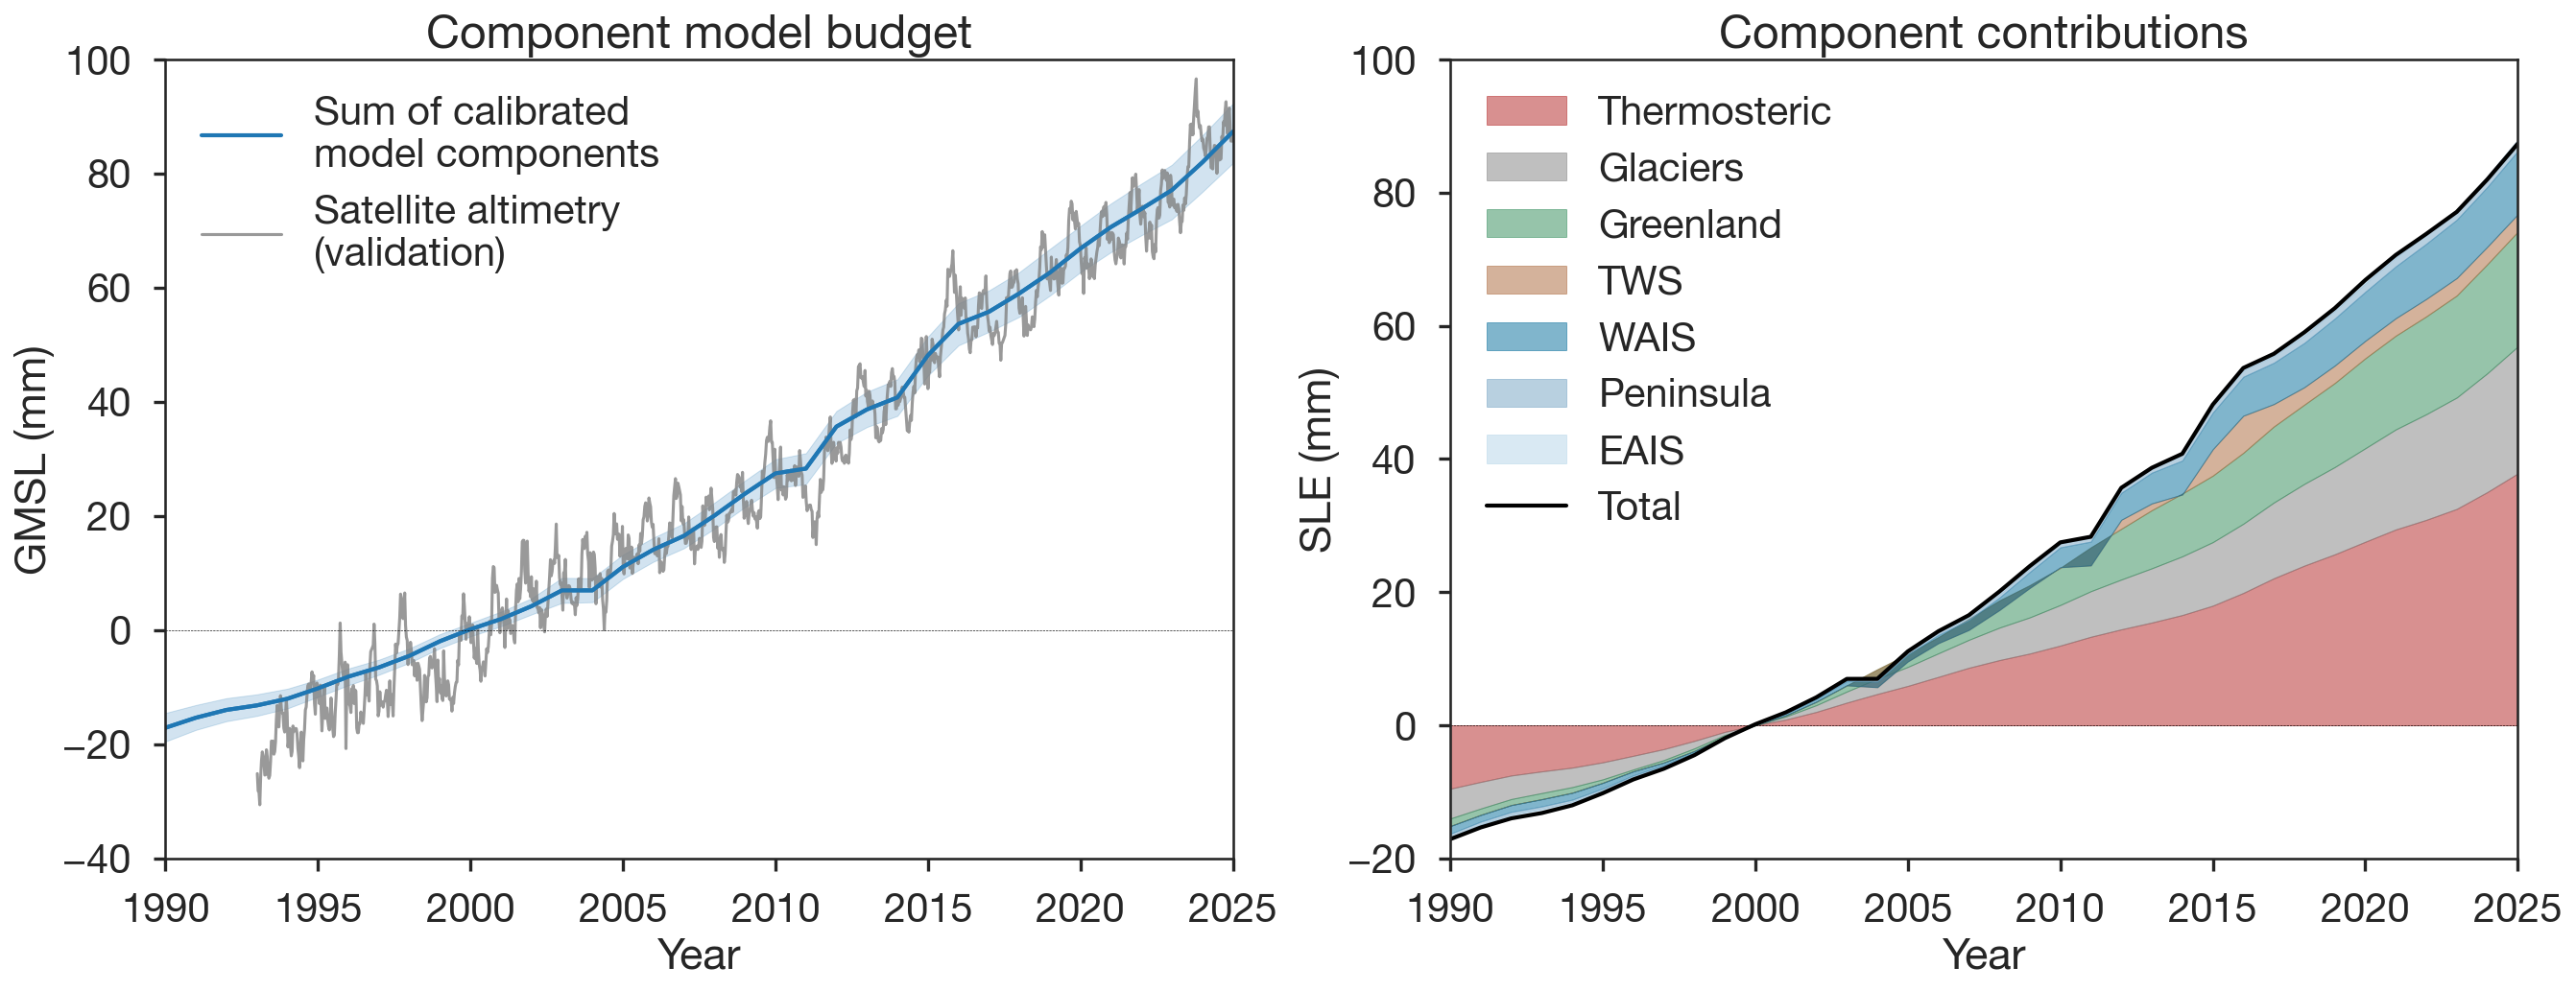
\includegraphics[width=\textwidth]{component_hindcast_vs_observed.png}
\caption{\textbf{Budget closure: temperature-forced component hindcast versus observed GMSL.}
\textbf{(A)}~Total component sum (red, with EAIS; orange dashed, without EAIS)
compared with NASA altimetry (black), Frederikse et~al.\ (blue), and
Dangendorf et~al.\ (grey) GMSL reconstructions.
\textbf{(B)}~Per-component contributions to the hindcast.
All values in mm relative to the year 2000 baseline.}
\label{fig:budget_closure}
\end{figure}

%% ================================================================
%% REFERENCES
%% ================================================================

\bibliographystyle{Science}
\bibliography{references}

\end{document}
